\begin{frame}{Overview}
\section{Implementation}
The model contain two main parts
\begin{itemize}
    \item Training Environment
    \item RL Model. 
\end{itemize}
\begin{center}
  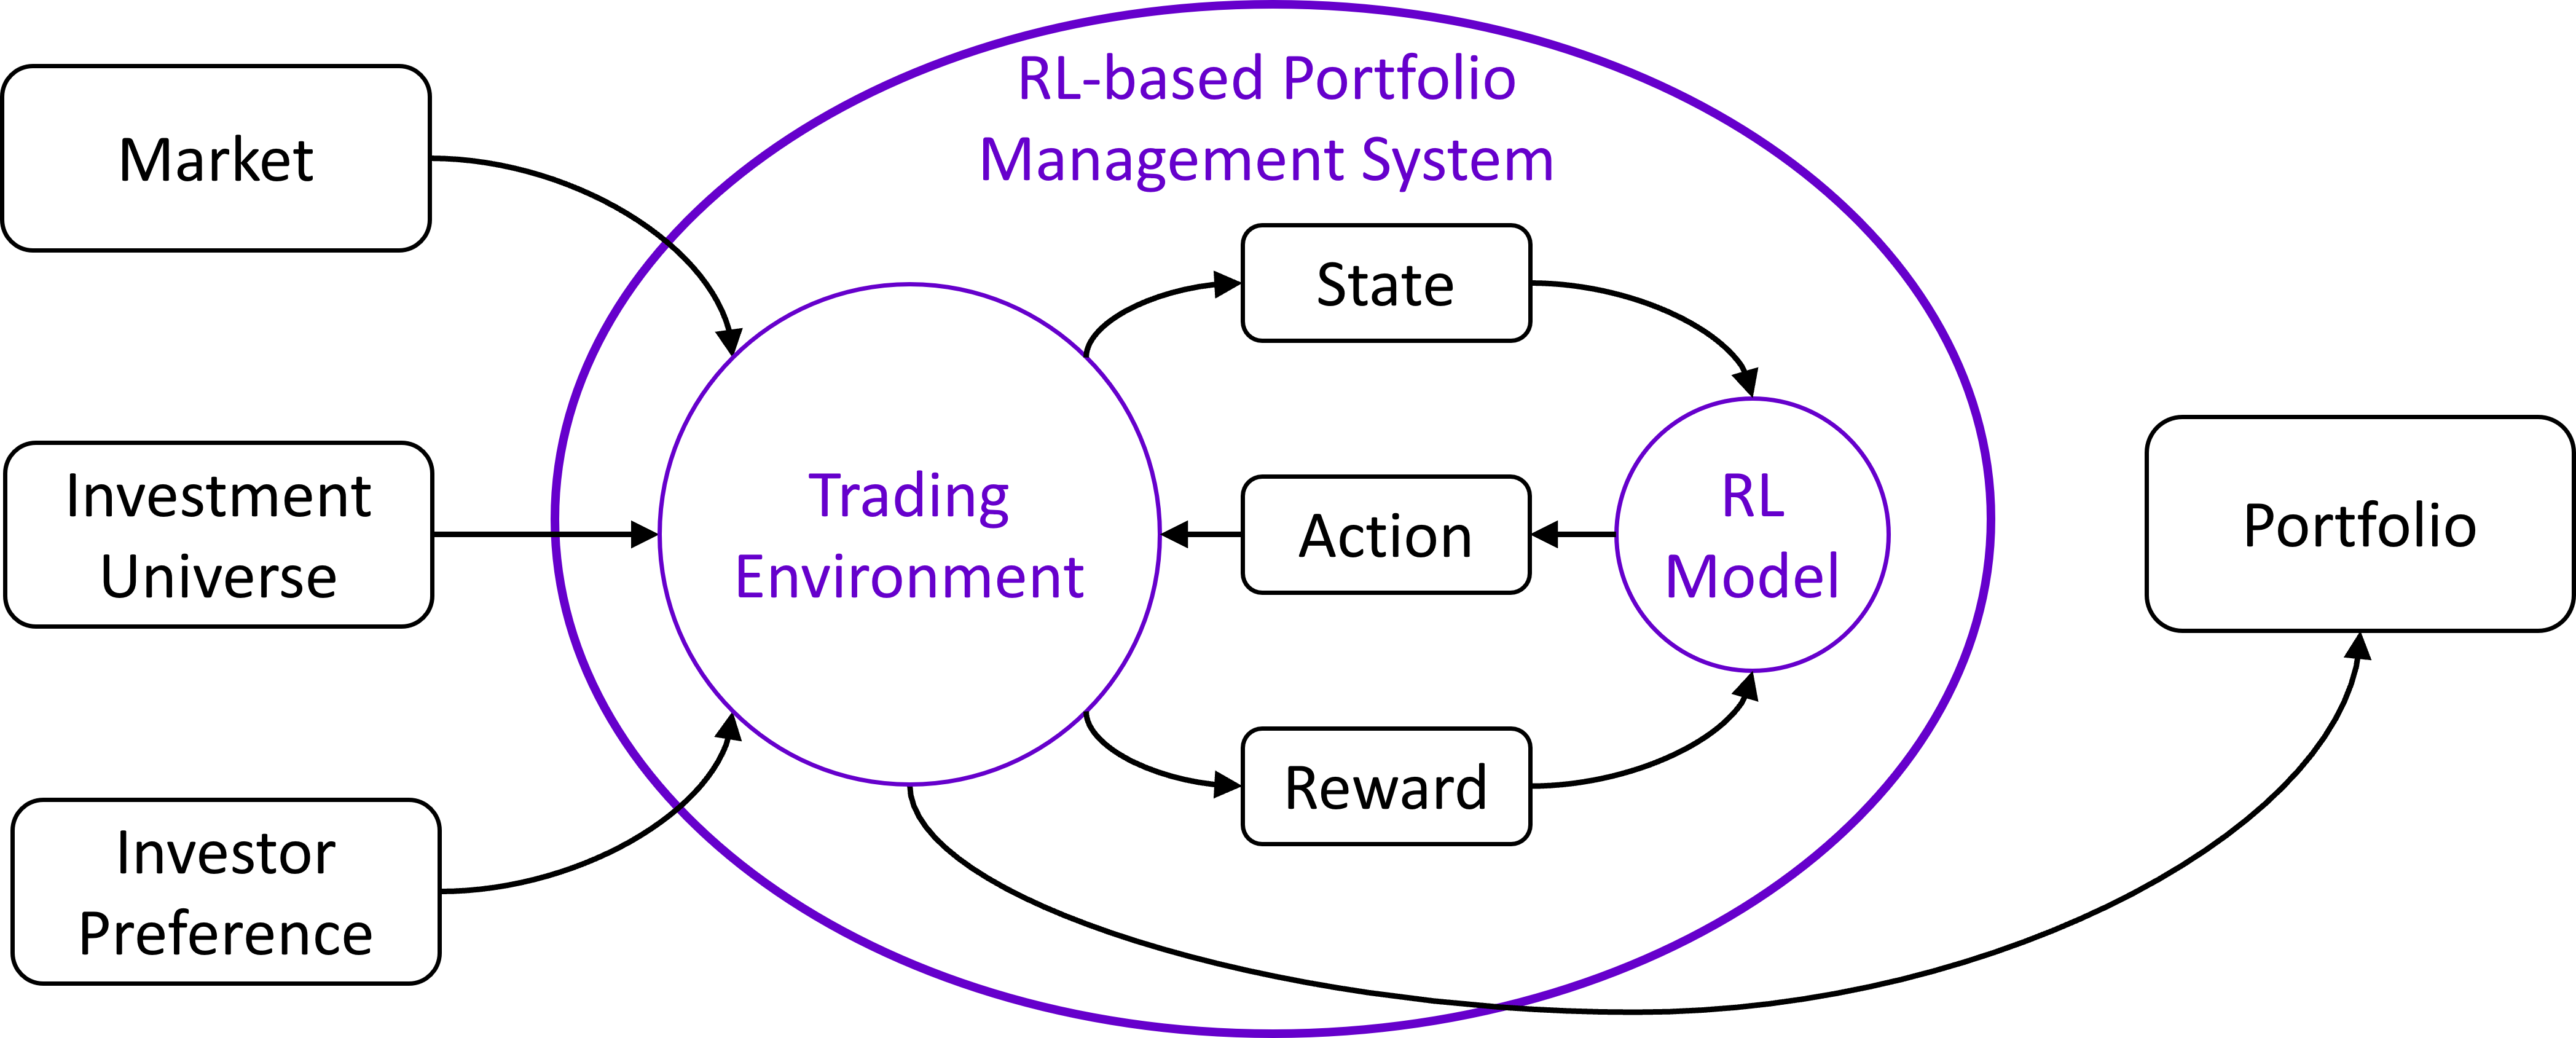
\includegraphics[width=10cm]{images/context_diagram.png}  
\end{center}
\end{frame}

\begin{frame}{Investment Universe}
\begin{block}{Goal}
Choose investments with low covariances between each other; hence their combinations can yield better profits from the same risk level
\end{block}
\par
\begin{block}{Number of investments}
\begin{itemize}
\item For stocks at least 30 or 40.

\item For ETFs, least than ten ETFs are sufficient to produce portfolios with adequate diversification
\end{itemize}
\end{block}

\end{frame}


\begin{frame}{Investments selection process}
    \begin{enumerate}
    \item Starts from the top 100 ETFs by Asset Under Management (AUM)
    \item Remove ones with trading records of less than 14 years.
    \item \label{itm:remove_items} Obtain the top two most correlated ETFs and remove the one with lower AUM
    \item Repeat Step\ref{itm:remove_items} iteratively until 10 ETFs are left
    \end{enumerate}
\end{frame}

\begin{frame}{Selection of ETFs}
    \begin{tabular}{|| c | c ||}
    \hline
    Symbol & Name  \\ \hline \hline
    SPY&SPDR S\&P 500 ETF \\ \hline
    AGG&iShares Core U.S. Aggregate Bond ETF \\ \hline
    BND&Vanguard Total Bond Market ETF \\ \hline
    GLD&SPDR Gold Trust \\ \hline
    LQD&iShares iBoxx \$ Investment Grade Corporate Bond ETF \\ \hline
    BSV&Vanguard Short-Term Bond ETF \\ \hline
    MBB&iShares MBS Bond ETF \\ \hline
    IGSB&iShares Short-Term Corporate Bond ETF \\ \hline
    SHY&iShares 1-3 Year Treasury Bond ETF \\ \hline
    SHV&iShares Short Treasury Bond ETF \\ \hline
    \end{tabular}
\end{frame}


\begin{frame}{Market Features}
\begin{block}{Structured information}
\begin{itemize}
    \item Interest rates
    \item Commodity prices
    \item Currency exchange indexes
\end{itemize}
\end{block}
\begin{block}{Stationary data}
   Use directly as features
\end{block}
\begin{block}{Non-stationary data}
    Use statistics measures among 5, 20, and 60 days as features, including standard deviation, skewness, and kurtosis.
\end{block}
\end{frame}

\begin{frame}{Market Features}
\begin{tabular}{|| c| c||}
\hline
Description & Categories \\ \hline \hline
5-Year Treasury Constant Maturity Rate & Interest Rates\\ \hline
10-Year Treasury Constant Maturity Rate & Interest Rates\\ \hline
30-Year Treasury Constant Maturity Rate & Interest Rates\\ \hline
5-Year Breakeven Inflation Rate & Interest Rates\\ \hline
10-Year Breakeven Inflation Rate & Interest Rates\\ \hline
Crude Oil Prices: Brent - Europe &  Commodities\\ \hline
Gold Prices &  Commodities\\ \hline
CBOE Volatility Index (VIX) &  Indexes\\ \hline
US Dollar Index (USDX) &  Currencies\\ \hline
\end{tabular}
\end{frame}


\begin{frame}{Investor Preference}
Risk aversion of the investors. 
Acquire risk aversion
Professional personnel or organization will acquire risk aversion from investors by survey or other techniques and interprets the inputs into comparable indicators between investors.

MDD as be 

\begin{block}{MDD}
One of the indicators to evaluate our system. However, optimizing any ratio using MDD directly has many problems and challenges. Some researches indicate MDDs are outliers or imply optimizing MDD is troublesome. Therefore, we will limit ourselves to use MDD while optimizing the model and consider other alternatives. 
\end{block}
\end{frame}



\begin{frame}{Reinforcement Learning Model}
\begin{block}{Overview}
Soft Actor-Critic (SAC) is an DRL algorithm
\begin{itemize}
    \item Optimizes a stochastic policy in an off-policy way
    \item Optimizes the policy with entropy regularization and takes entropy, measuring randomness in the policy, into account.
\end{itemize}
\end{block}
\begin{block}{Reward Scale}
SAC is highly sensitive to the scaling of the reward. 
\begin{itemize}
    \item If reward scale is too small, the reward will fail to affect the model, and the policy will become nearly uniform.
    \item If reward scale is too large, the model will learn quickly and become deterministic, leaving no room for exploration.
\end{itemize}
\end{block}
\end{frame}



\begin{frame}{Trading Environment}
A trading environment compatible with Open AI Gym
\begin{center}
  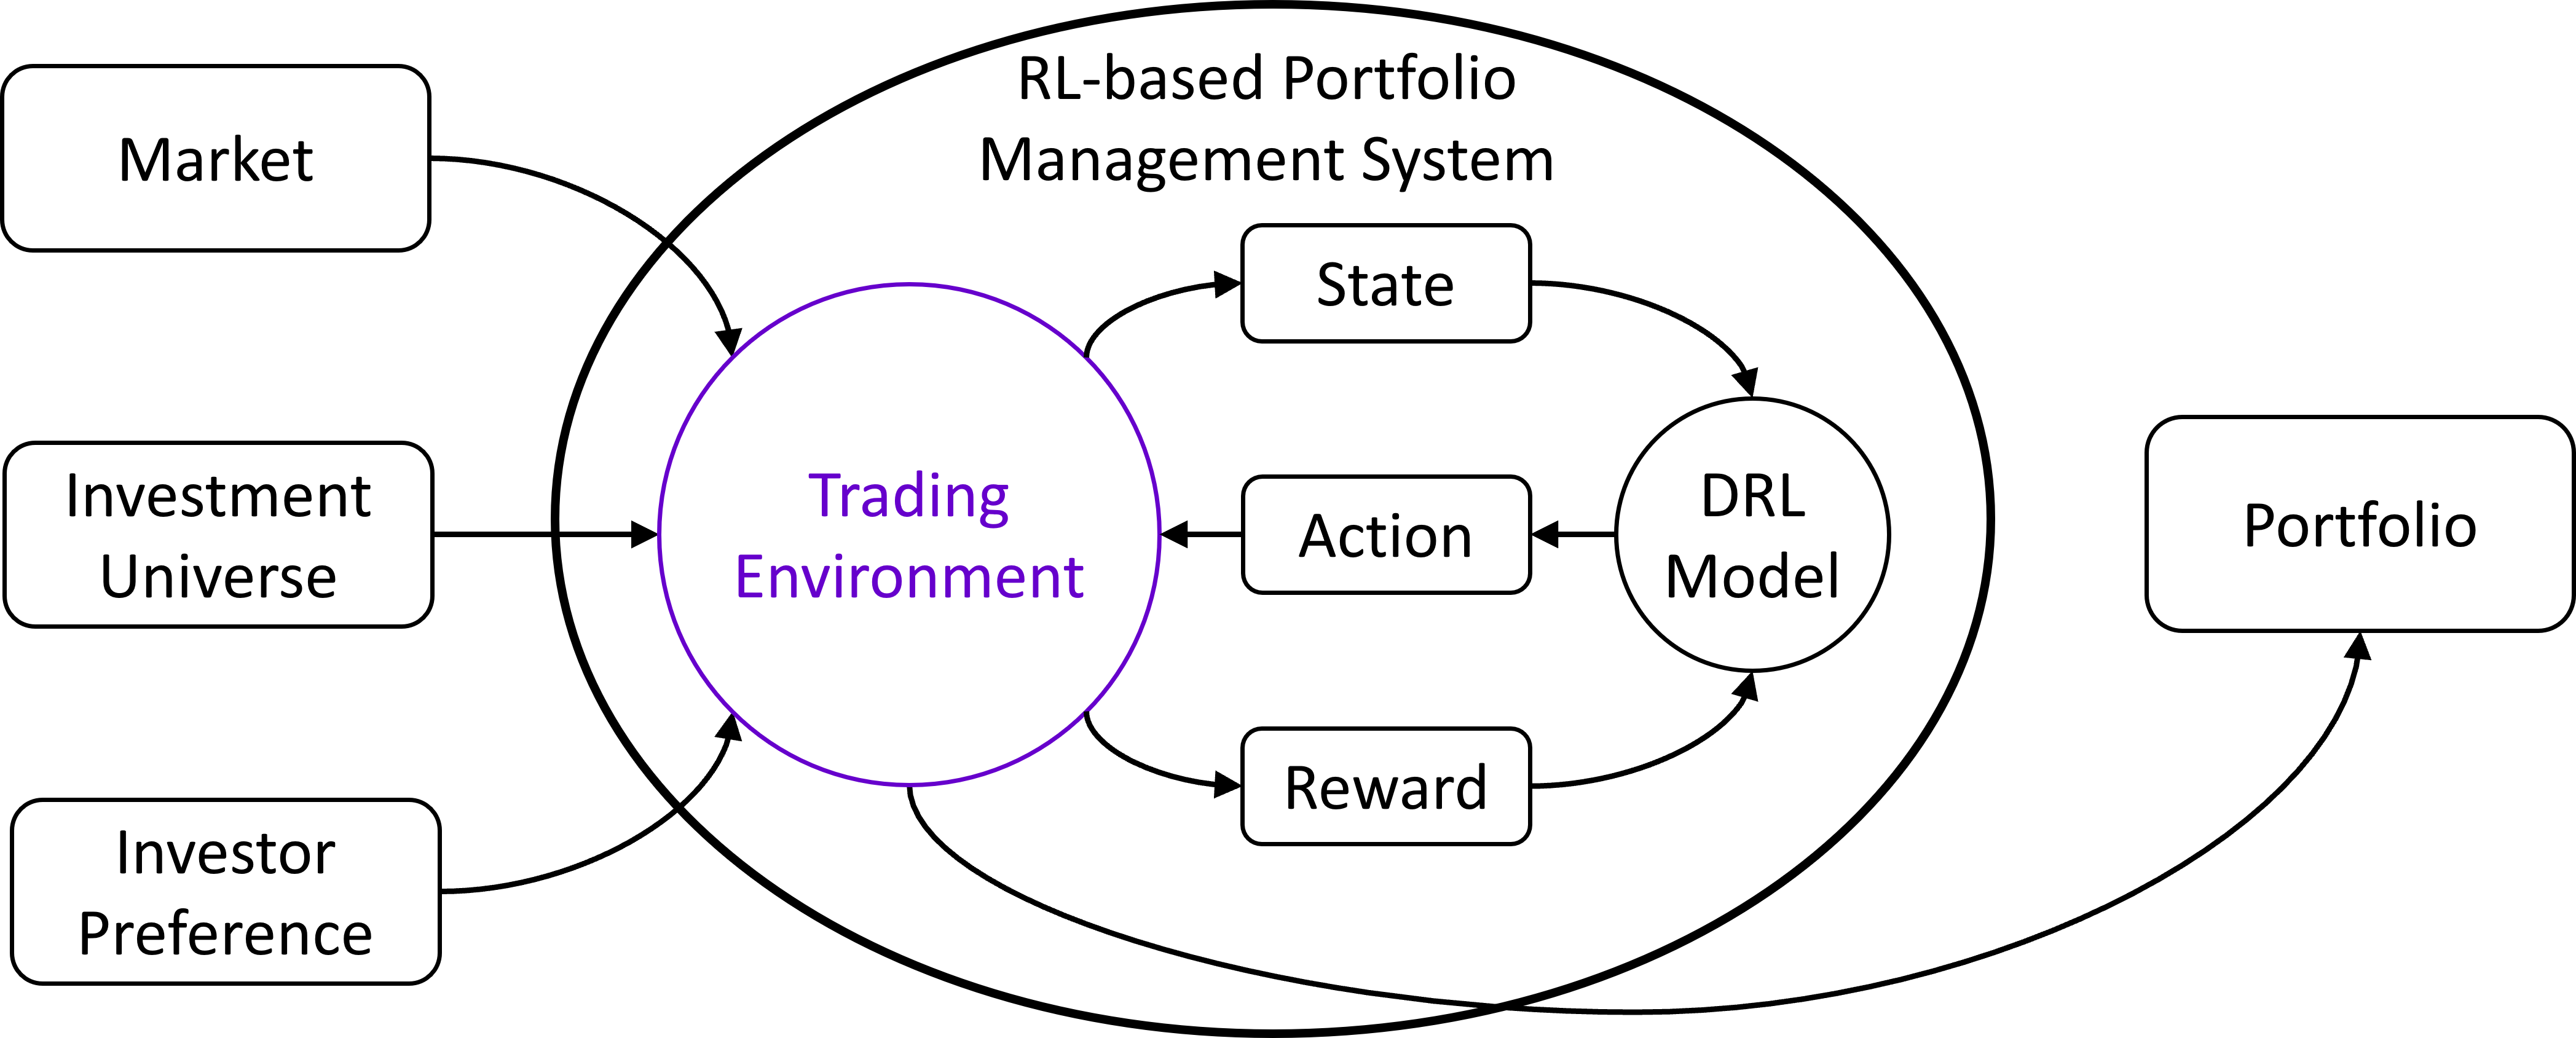
\includegraphics[width=10cm]{images/trading_environment.png}
\end{center}
\end{frame}

\begin{frame}{Feature Extractor}
\begin{center}
  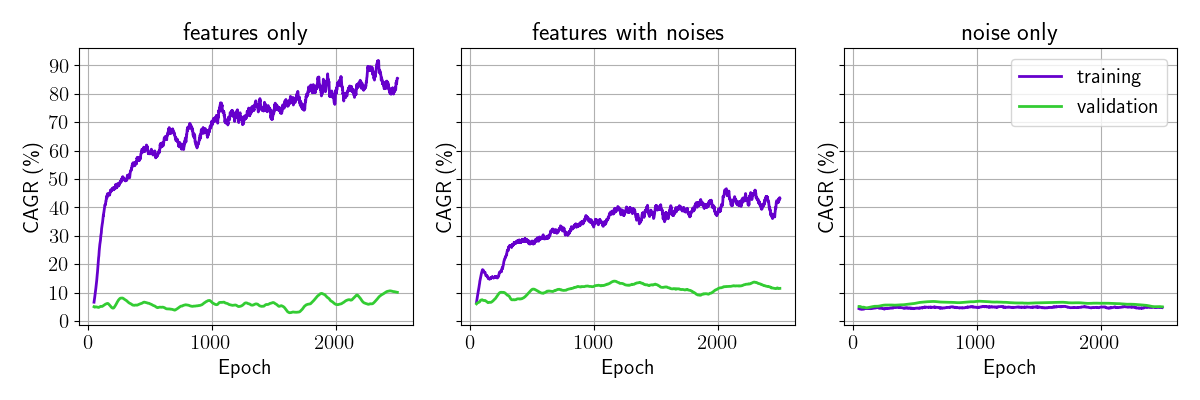
\includegraphics[width=10cm]{images/compare_noise.png}
\end{center}
\end{frame}

\begin{frame}{Portfolio Builder}
The portfolio builder builds the portfolio from the investible universe and the action from the RL model.
The portfolio F contains no short position and is an m dimension vector space of weights w, a real number between 0 and 1. , where m is the number of investments in the investment universe. Wealth will all be in the form of investments, so the sum of the weights will equal 1.
\[
    F = \{ {f \in \mathbb{R} | 0 \leq f \leq 1 } \} ^m,
    \sum_{i=1}^m {f_i} =1
\]
We distribute the weight based on the action proportionally.
\[
    F_i = \cfrac{a_i}{\sum a} 
\]
where \(F_i\) is the weight for \(i^{th}\) investment, \(a_i\) is the  \(i^{th}\) action, m is the total number of investments in the investible universe. 

\end{frame}


\begin{frame}{Trading System}
Measures performances of the given portfolios
\begin{itemize}
    \item MDD
    \item CAGR
    \item profit
    \item wealth
\end{itemize}
These performances will be the input to calculate the reward or evaluate the performance of the system. 
    
\end{frame}

\begin{frame}{Reward Provider}
We first use profit p as the baseline for the reward and add a penalty, \(p_t-\theta\), upon negative profits exceeding the given absolute value threshold \(\theta\). 
\[
p_t = \frac{w_t-w_{t-1}}{w_{t-1}}
, 
R_t = 
\begin{cases}
    p_t,&\text{if  }p_t > -\theta\\
    2p_t - \theta ,&\text{if  }p_t \leq  \theta
\end{cases}
\]
where \(R_t\) is the reward, \(p_t\) is the profit and \(w_t\) is the wealth on given t.
\\
On all threshold \(\theta\) given, the result shows unstable improvement in MDD. We observed that the optimization goes too well during training and generates a tiny amount of negative profits; therefore, these negative profits have minimal penalty effect on the model parameters.
\\

\end{frame}

\begin{frame}{Reward Provider}
We then apply the penalty upon both positive and negative profits. This increases the stability significantly.
\[
R_t = 
\begin{cases}
    2p_t - \theta,&\text{if  }    $$|p_t|$$ > \theta\\
    p_t - \theta ,&\text{if  } $$|p_t|$$\leq  \theta
\end{cases}
\]
The threshold \(\theta\) will be the main adjustable parameter of our system. Adjusting it will enable the system to produce portfolios to meet different investors' risk tolerance.
\end{frame}
\begin{frame}{Reward Provider}
\begin{center}
      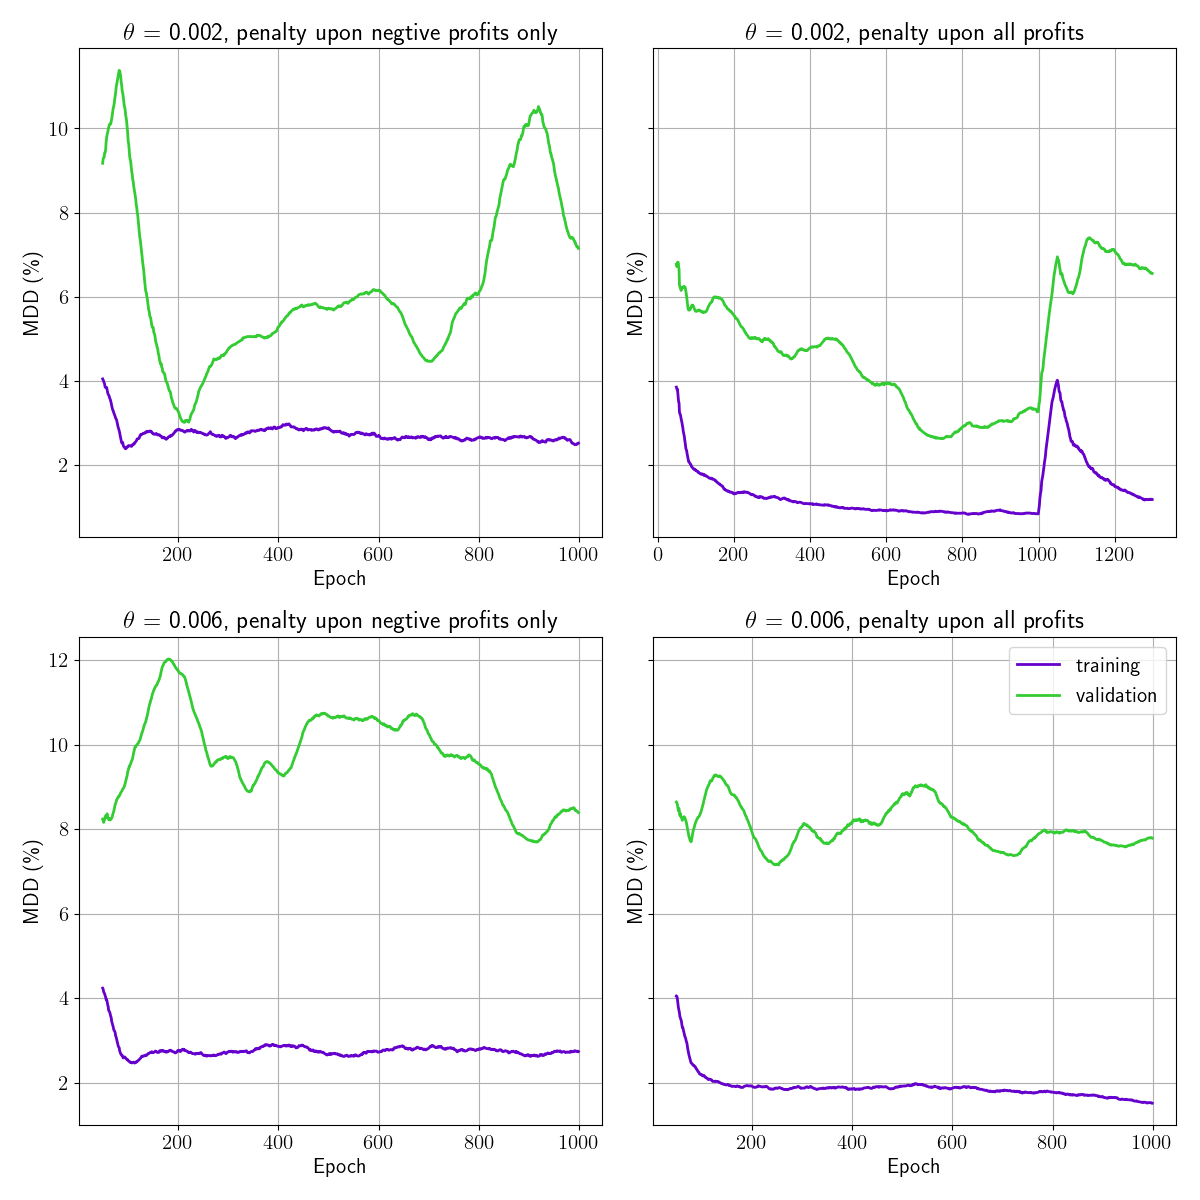
\includegraphics[height=7cm]{images/penalty_negtive_profits_compare.png}
\end{center}
\end{frame}

\begin{frame}{Result}
\begin{center}
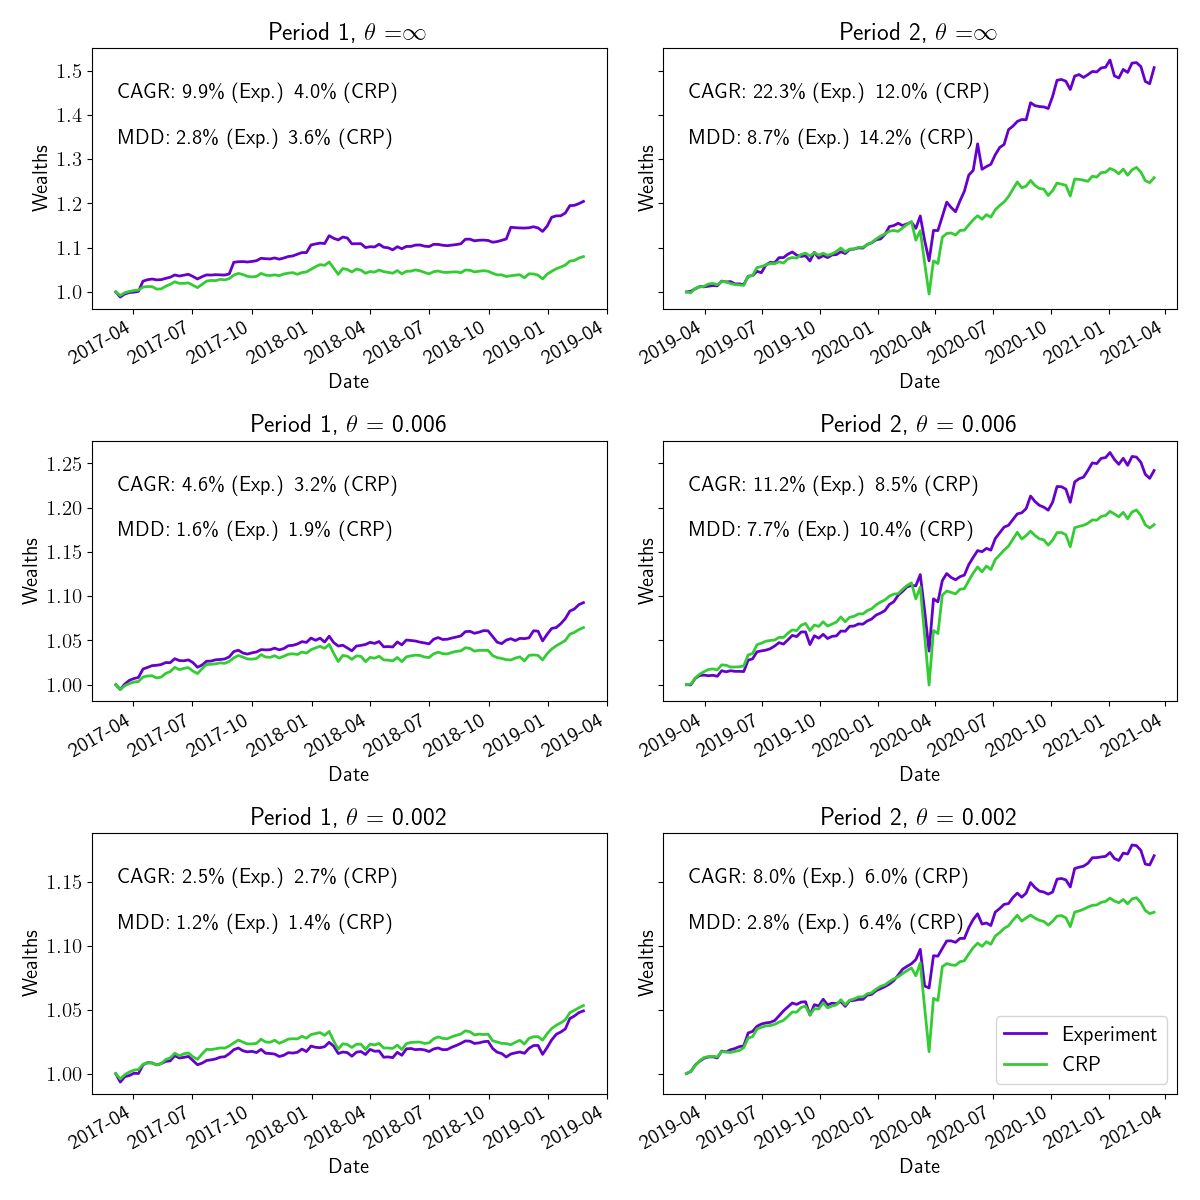
\includegraphics[height= 7.5cm]{images/crp_compare.png}
\end{center}
\end{frame}
